 \documentclass[12pt]{report}
% ---------------------- Required Packages ----------------------
\usepackage{Styles/GUB}               % Custom style

\usepackage[english]{babel}          % English language
\usepackage{graphicx}                % Graphics inclusion
\usepackage{caption}
\usepackage{subcaption}             % Subfigures
\usepackage{float}                  % For forcing table/figure position
\usepackage{amsmath, amssymb, amsfonts} % Math packages
\usepackage{bm}                     % Bold math
\usepackage{mathptmx}               % Times font
\usepackage{siunitx}                % SI units
\usepackage{array}                  % Extended tables
\usepackage{longtable}
\usepackage{adjustbox}
\usepackage{booktabs}               % Better tables
\usepackage{multirow}
\usepackage{tabularx}               % Tables with flexible columns
\usepackage[table]{xcolor}
\usepackage{url}                    % Format URLs
\usepackage{xcolor}                 % Colored text


% Please add the following required packages to your document preamble:
% \usepackage{multirow}
\usepackage[table,xcdraw]{xcolor}
%\usepackage{colortbl}
\usepackage{pdflscape}
\usepackage[normalem]{ulem}
\useunder{\uline}{\ul}{}
\usepackage{lipsum}                 % Dummy text
\usepackage{fancyhdr}               % Fancy headers
\usepackage{epstopdf}               % EPS support
\usepackage{enumerate}              % Custom enumeration
\usepackage[utf8]{inputenc}


\usepackage{hyperref}
\hypersetup{
    colorlinks=true,
    linkcolor=magenta,
    citecolor=magenta,
    urlcolor=magenta,
    filecolor=magenta
}

\usepackage[a4paper, left=1.5in, right=1in, bottom=1.3in]{geometry}

\usepackage{ragged2e}
\usepackage[utf8]{inputenc}

\hypersetup{colorlinks=true, linkcolor=black, filecolor=magenta, urlcolor=cyan}
\usepackage[nottoc,notlof,notlot]{tocbibind} 
\usepackage{pifont}                 % Special symbols
\usepackage{lscape}                 % Landscape tables
\usepackage{mwe}                    % Example images
\usepackage{nomencl}                % List of symbols
\usepackage{algorithm2e}            % Algorithms
\usepackage{epsfig}                 % EPS figures (if needed)
\usepackage{listings}

% \usepackage{tikz}
% \usetikzlibrary{arrows,positioning}
% \usetikzlibrary{positioning}


\lstset{
    basicstyle=\ttfamily\small,
    keywordstyle=\color{blue},
    commentstyle=\color{gray},
    stringstyle=\color{purple},
    showstringspaces=false,
    breaklines=true,
    frame=single
}


\lstdefinestyle{tree}{
  basicstyle=\ttfamily\small,
  backgroundcolor=\color{gray!5},
  frame=single,
  breaklines=true,
  showstringspaces=false
}

\lstdefinestyle{bash}{
    backgroundcolor=\color{gray!10},
    basicstyle=\ttfamily\footnotesize,
    frame=single,
    breaklines=true,
    showstringspaces=false,
    language=bash
}

% ---------------------- Algorithm2e Settings ----------------------
\SetKwInput{KwInput}{Input}
\SetKwInput{KwOutput}{Output}
\newcommand\mycommfont[1]{\footnotesize\ttfamily\textcolor{blue}{#1}}
\SetCommentSty{mycommfont}
\SetAlgoNlRelativeSize{0}

% ---------------------- General Settings ----------------------
\renewcommand{\baselinestretch}{1.5}
\pagestyle{plain}
\renewcommand{\labelenumi}{\alph{enumi}.}

% ---------------------- Column Types for Tables ----------------------
\newcolumntype{C}{>{\raggedright\arraybackslash}p{18em}}
\newcolumntype{D}{>{\raggedleft\arraybackslash}p{15.5em}}

\begin{document}

% ---------------------- Front Matter ----------------------
\begin{titlepage}
\begin{center}

% YOU MUST ENSURE THAT THE GUB LOGO AND COMPANY LOGO ARE PROPERLY ALIGNED

% --- Logos Row ---
% \vspace{0.0cm}

\begin{figure}[h!]
    \centering
    \begin{subfigure}[b]{0.3\textwidth}
        \centering
        
\includegraphics[width=0.8\textwidth]{figures/GUBLogoNew.png}
    \end{subfigure}
    \hfill
    \begin{subfigure}[b]{0.3\textwidth}
        \centering
        
\includegraphics[width=0.8\textwidth]{figures/wecycle_logo.png}
    \end{subfigure}
\end{figure}

\vspace{0.6cm}

% --- University Name ---
{\Large \textbf{GREEN UNIVERSITY OF BANGLADESH}}

\vspace{0.6cm}

% --- Report Title ---
\textbf{Industrial Training}\\
\vspace{0.2cm}
\textbf{on}\\
\vspace{0.2cm}
\textbf{Full-Stack Web Development}

\vspace{1.5cm}

% --- Submitted by ---
\textbf{Submitted by}\\
Jubaer Al Mamun – 221902013

\vspace{0.8cm}

% --- Submission Purpose ---
\begin{minipage}{1\textwidth}
\centering
\textit{An industrial training report submitted to the Department of Computer Science \& Engineering, for the partial fulfillment of the degree of Bachelor of Science in Computer Science \& Engineering}
\end{minipage}

\vspace{0.8cm}

% --- Supervisor Info ---
\textbf{Under the Supervision of}\\
Md. Parvez Hossain\\
Lecturer, Department of CSE

\vspace{0.8cm}

% --- Training Place Info ---
% --- Training Place Info ---
\textbf{Training Place}\\
Tanbel Inc. (Parent of WeCycle)\\
United States (Remote)

\vspace{0.8cm}

% --- Details Table ---
\begin{tabular}{@{}ll}
\hspace{1.8cm}\textbf{Training Duration    :} & 13.10.2025 to 05.12.2025 \\
\hspace{1.8cm}\textbf{Industrial Supervisor      :} & MD Tanvir Ahmed \\
% \hspace{1.8cm}\textbf{Academic Supervisor      :} & Supervisor Name \\
\hspace{1.8cm}\textbf{Report Submission Date          :} & 26.12.2025 \\
\end{tabular}'

\vspace{0.7cm}
{\Large \textbf{Fall 2025}}

% \begin{center}
% \end{center}
% \thispagestyle{empty}
% \vspace*{\fill}
% \vspace*{\fill}

\end{center}
\end{titlepage}

\pagenumbering{roman}
\chapter*{\centering Declaration}
\addcontentsline{toc}{chapter}{Declaration}

Declaring this training report to be founded only on my own research results, I make it clear. References are made to research materials discovered by other researchers. This work has not been submitted for a degree before, either in full or in part.


\bigskip
\bigskip
\bigskip


\begin{tabular}{p{5cm}p{5cm}p{5cm}}
\centering
  % after \\: \hline or \cline{col1-col2} \cline{col3-col4} ...
     &  &   \\
     &  &   \\
     &  &   \\
 \rule{4cm}{1pt} 
 \\
  Jubaer Al Mamun \\
  ID: 221902013

  
\end{tabular}
\chapter*{\centering Certificate}
\addcontentsline{toc}{chapter}{Certificate}

This is to certify that the industrial training report entitled \textit{Full-Stack Web Development} has been prepared and submitted by \textbf{Jubaer Al Mamun} in partial fulfillment of the requirements for the degree of Bachelor of Science in Computer Science and Engineering on 26 December 2025.

\bigskip
\bigskip
\bigskip
\bigskip

\noindent
\begin{tabular}{p{7cm} p{2cm} p{7cm}}
  \rule{6cm}{1pt} & & \rule{5cm}{1pt} \\
  Md. Parvez Hossain  & & MD Tanvir Ahmed \\
  Academic Supervisor & & Industrial Supervisor \\
  Green University of Bangladesh & & Tanbel Inc. \\
\end{tabular}

\bigskip
\noindent
\begin{center}
    \vspace{0.5cm}
    \textit{Accepted and approved in partial fulfillment of the requirements for the degree\\
    Bachelor of Science in Computer Science and Engineering.}
    \vspace{0.5cm}
\end{center}

\noindent
\begin{tabular}{p{6cm} p{3cm} p{6cm}}
  &  &  \\
  &  &  \\
  \rule{6cm}{1pt} &  & \\
  Chairman \\ \\
  &  &  \\
  \rule{5cm}{1pt} &  & \rule{5cm}{1pt} \\
  Board Member & & Board Member \\
\end{tabular}

\chapter*{\centering Acknowledgments}
\addcontentsline{toc}{chapter}{Acknowledgments}

I would like to express my sincere gratitude to all those who supported and guided me throughout the industrial training period from \textbf{October 13, 2025} until \textbf{December 5, 2025}. Their encouragement and assistance were invaluable, especially during times when I faced challenges.

I am thankful to my academic supervisor, \textbf{Md. Parvez Hossain, Lecturer, Department of CSE, Green University of Bangladesh}, for providing consistent guidance and support during the training. Their feedback and suggestions helped me stay focused and improved the overall quality of my learning experience.

I am also grateful to the professionals at \textbf{Tanbel Inc.} (specifically the \textbf{WeCycle} team), especially my industrial supervisor \textbf{MD Tanvir Ahmed}, for their valuable insights, technical guidance, and for sharing their industry experience. Their support greatly enhanced my understanding of real-world practices in \textbf{Full-Stack Web Development}, modern JavaScript frameworks, and agile work culture.

I would also like to acknowledge the entire development team at WeCycle for their patience in reviewing my code, providing constructive feedback, and helping me understand the complexities of working with large-scale web applications.

Finally, I would like to thank my family and friends for their constant encouragement, emotional support, and motivation, which played a vital role in helping me successfully complete the training.

\bigskip

% Note: Remove the blue text below before final submission
% \textcolor{blue}{\textbf{This internship report follows the template structure provided by the Department of CSE, Green University of Bangladesh.}}
\chapter*{\centering Abstract}
\addcontentsline{toc}{chapter}{Abstract}

\par
This report summarizes the industrial training experience completed at \textbf{Tanbel Inc.}, a US-based technology company. The training utilized their two primary products: \textbf{WeCycle} (\href{https://getwecycle.com/}{https://getwecycle.com/}), a B2C junk removal service, and \textbf{ArrayQ} (\href{https://arrayq.com/}{https://arrayq.com/}), a B2B hauler dashboard CRM solution. The training focused on the practical application of \textbf{Full-Stack Web Development} and mobile application maintenance. The primary objective was to gain hands-on experience in developing scalable user interfaces and backend integrations for large enterprise applications.
\par
The training involved working with a modern technology stack, including \textbf{React.js, Next.js, TypeScript, Tailwind CSS, Capacitor, and Docker}. Industry-standard tools like \textbf{Jira} for project management and \textbf{GitHub} for version control were integral to the daily workflow.
\par
Key contributions included \textbf{developing the ArrayQ landing page and mobile app features, implementing a complex invoice and payment system using Stripe, integrating an AI-powered chatbot for customer support, and migrating legacy Ant Design components to a custom UI library}. Extensive work was also done on optimizing the \textbf{WeCycle Dashboard} for iPad and tablet devices, fixing critical bugs, and setting up staging environments for rigorous testing.
\par
This internship provided a comprehensive learning experience, bridging the gap between academic theory and professional software engineering. It offered deep insights into agile development cycles, code quality standards, and the operational dynamics of a remote tech startup, preparing me for a career as a \textbf{Full-Stack Developer}.

\vspace{0.5cm}

\noindent\textbf{Keywords:}
Tanbel Inc., WeCycle, ArrayQ, React.js, Next.js, TypeScript, Docker, Stripe


\tableofcontents
\newpage
\listoffigures
\addcontentsline{toc}{chapter}{List of Figures}
\newpage
\listoftables
\addcontentsline{toc}{chapter}{List of Tables}

% ---------------------- Main Matter ----------------------
\newpage
\pagenumbering{arabic}
\setcounter{page}{1}

\chapter{Introduction}

\par The transition from academic theory to professional engineering is often abrupt. While university courses provide a strong foundation in algorithms and syntax, they rarely simulate the volatility of a production environment. In a classroom, code is written to pass test cases; in the industry, code is written to survive user interaction, scalability demands, and market pivots. This industrial training at \textbf{Tanbel Inc.} was not just an application of skills—it was an immersion into the reality of modern software development. I moved from writing isolated functions to contributing to a living, breathing product ecosystem, where "urgent" means "now," and stability is the primary metric of success.

\par The objective of this training was to bridge the gap between student mindset and engineer mindset. It required navigating complex codebases, understanding the business logic behind B2C and B2B operations, and delivering features that directly impacted the company's bottom line.

\section{Problem Domain}

\par \textbf{Tanbel Inc.} operates at the intersection of logistics and waste management—an industry traditionally bogged down by manual processes and paper trails. The problem is coordination: connecting customers who need junk removed with haulers who have the capacity to remove it, instantly and reliably.

\par To solve this, Tanbel Inc. deploys two flagship products:
\begin{itemize}
    \item \textbf{WeCycle} (\href{https://getwecycle.com/}{getwecycle.com}): A B2C platform that allows homeowners and businesses to book junk removal services on-demand. Think of it as the "Uber" for junk.
    \item \textbf{ArrayQ} (\href{https://arrayq.com/}{arrayq.com}): A B2B CRM and dashboard solution designed for haulers to manage their dumpsters, inventory, and schedules efficiently.
\end{itemize}

\par My role as a \textbf{Full-Stack Developer} was to maintain and enhance the digital infrastructure that powers these solutions. Specifically, I worked on the WeCycle Dashboard Application (WCAPP) and the ArrayQ mobile/web platforms, ensuring that the connection between the customer’s request and the hauler’s execution was seamless.

\par As a trainee, I didn’t just watch; I had to get my hands dirty. I ran into a bunch of hurdles:
\begin{itemize}
    \item We had to rip out the old Ant Design components and replace them with our custom web-ui library. It was tedious, but necessary.
    \item I had to make the WCAPP look good on everything—phones, tablets, desktops. If it looked bad on an iPad, it was my problem.
    \item Debugging state management in a massive app is... painful. But I had to figure it out.
    \item I also had to learn the codebase without breaking it. It’s intimidating to push code to a repo that people actually depend on.
\end{itemize}

\par I couldn't have done it alone. My team—supervisors and colleagues—were a huge help. We used the modern stack: React.js, Next.js, and TypeScript. Honestly, it’s the standard now for a reason.

\section{Motivation of Training}

\par Why did I do this? A few reasons:

\begin{itemize}
    \item \textbf{Actually Using What I Learned:} I wanted to see if the software engineering theories I sat through in class actually hold up. (Spoiler: Some do, some don't.)
    \item \textbf{Getting Better, Faster:} I needed to get sharp with React.js and Next.js. TypeScript was another beast I wanted to tame.
    \item \textbf{Agile Chaos:} I wanted to see what "Agile" feels like when deadlines are real.
    \item \textbf{Meeting People:} It’s not just about code. I wanted to meet developers who have been doing this for years and pick their brains.
    \item \textbf{Future-Proofing:} I’m trying to build a career here. This was the groundwork.
\end{itemize}

\section{Training Goals}

\par My goals were pretty straightforward:

\begin{itemize}
    \item Get really, really good at React.js and Next.js.
    \item Stop solving textbook problems and start solving business problems.
\end{itemize}

\section{Scope of Training}

\section{Scope of Training}

\par My role was multifaceted, operating across the entire application stack. As a \textbf{Full-Stack Developer}, I was responsible for end-to-end feature delivery—from designing database schemas to deploying pixel-perfect UIs.

\par The scope included:
\begin{itemize}
    \item \textbf{Frontend Engineering:} Building responsive interfaces with React.js, Next.js, and Capacitor for mobile.
    \item \textbf{Backend Development:} Architecting scalable APIs using Node.js and Express.js, and managing data integrity with MongoDB and PostgreSQL.
    \item \textbf{DevOps \& Infrastructure:} Configuring Docker containers, managing Nginx servers, and optimizing CI/CD workflows with Nx and GitHub Actions.
    \item \textbf{System Integration:} Connecting third-party services like Stripe (payments) and AI bots to the core platform.
\end{itemize}

\par I did not stay in a single lane. If a feature required a database migration, I wrote it. If the build pipeline failed, I fixed it. This holistic approach allowed me to understand the software lifecycle in its entirety.

\section{The Reality Check: Academia vs. Industry}

\par There is a massive disconnect between what you learn in school and what you do at work. Here’s the truth:

\begin{itemize}
    \item \textbf{Theory vs. Reality:} School teaches you the syntax; work teaches you the context. Knowing *how* to write a loop is easy. Knowing *where* to put it so it doesn't crash the browser is harder.
    \item \textbf{Tooling Shock:} In university, you maybe use Git once. In the industry, if you don't know Git, Jira, or how to read a PR, you're useless.
    \item \textbf{The Human Factor:} School projects are usually solo or with friends. Real work is collaborating with people who might disagree with your code style.
    \item \textbf{Messy Constraints:} In class, you have all semester. In work, you have until Friday, and the specifications just changed this morning.
    \item \textbf{Legacy Code:} School start projects from scratch (file -> new). Work involves staring at 5-year-old code and trying to figure out what the original developer was thinking.
\end{itemize}

\section{Pain Points \& Growth}

\subsection{The Hard Stuff (Challenges)}
\begin{itemize}
    \item Jumping into a massive codebase is terrifying. You feel like you know nothing.
    \item Balancing "make it perfect" with "get it done" is a constant struggle.
    \item Refactoring old components without breaking everything else is stressful.
    \item Keeping up with the sprint pace—it’s fast.
    \item CSS media queries are finicky.
\end{itemize}

\subsection{Where I Grew}
\begin{itemize}
    \item My React/Next.js skills are night-and-day better.
    \item I learned how to actually manage my time.
    \item I'm comfortable with the tools now—VS Code and I are best friends.
    \item I learned how to take feedback on my code without taking it personally.
    \item I can actually debug things now instead of just staring at the screen.
\end{itemize}

\section{Detailed Plan}

\par I was at \textbf{Tanbel Inc.} from \textbf{October 13, 2025} to \textbf{December 5, 2025}. I didn't just sit around; I was busy.

\subsection{Resources}

\begin{enumerate}
    \item \textbf{People:} MD Tanvir Ahmed (my supervisor) and the other devs were lifesavers. Code reviews were where the real learning happened.
    \item \textbf{Technical Resources:} Access to development tools including Visual Studio Code, Git/GitHub, Chrome DevTools, Jira for task management, and the company's internal component libraries and design systems.
\end{enumerate}

\subsection{Timeline}

\par Here is exactly what I did, week by week. It was a busy two months.

\begin{table}[H]
\centering
\caption{Project Timeline Planning - Weekly Task Distribution}
\label{tab:training_timeline}
\resizebox{\textwidth}{!}{%
\begin{tabular}{|p{5.5cm}|c|c|c|c|c|c|c|c|}
\hline
\textbf{Tasks} & \textbf{Wk 1} & \textbf{Wk 2} & \textbf{Wk 3} & \textbf{Wk 4} & \textbf{Wk 5} & \textbf{Wk 6} & \textbf{Wk 7} & \textbf{Wk 8} \\
\hline
Env Setup \& CI/CD Optimization & \checkmark & & & & & & & \\
\hline
Mobile App Navigation \& UI Fixes & \checkmark & & & & & & & \\
\hline
Chatbot Service Deployment & & \checkmark & & & & & & \\
\hline
Staging Database \& Env Config & & \checkmark & & & & & & \\
\hline
Invoice \& Booking Logic Fixes & & & \checkmark & & & & & \\
\hline
CSV Export & Hauler Details Impl. & & & \checkmark & & & & \\
\hline
ArrayQ Site Deployment & Branding & & & & \checkmark & & & \\
\hline
Blog Page \& Dynamic Content Caching & & & & & \checkmark & & & \\
\hline
Blog Fixes \& App Store Review & & & & & & \checkmark & & \\
\hline
Mobile App Pricing & Discount Fixes & & & & & & \checkmark & \\
\hline
Stripe Connect \& Subscription Features & & & & & & & & \checkmark \\
\hline
Final Testing \& Documentation & & & & & & & & \checkmark \\
\hline
\end{tabular}%
}
\end{table}

\section{Risk Analysis: What Could Go Wrong?}

\begin{itemize}
    \item \textbf{Technical Challenges:} Sometimes I got stuck. The fix? Ask for help, read the docs, try again.
    \item \textbf{Timeline Risks:} Sprints move fast. I had to break tasks down so I didn't drown.
    \item \textbf{Communication Barriers:} Remote work is hard. Slack and Google Meet were the lifelines.
    \item \textbf{Quality:} We tested everything. I didn't want to be the guy who broke production.
\end{itemize}

\section{Report Outline}

\begin{itemize}
    \item \textbf{Chapter 2:} Who is \textbf{WeCycle}? The organization structure and mission.
    \item \textbf{Chapter 3:} What I actually did—tools and workflows.
    \item \textbf{Chapter 4:} The skills—what I learned.
    \item \textbf{Chapter 5:} Final thoughts—the conclusion.
    \item \textbf{Chapter 6:} Mapping outcomes (The official stuff).
    \item \textbf{Chapter 7:} SDG Goals (Sustainability mapping).
    \item \textbf{Chapter 8:} Appendix—The weekly logs.
\end{itemize}

\section{Conclusion}

\par This wasn't just an internship. It was a reality check. WeCycle didn't hold my hand; they let me work. I wrote real code for real users, and that changes how you think. It’s one thing to pass an exam. It’s another to fix a bug while your project manager is waiting. Honestly? I learned more here in a few weeks than I did in years of lectures. I’m not just ready to work. I’m ready to solve problems.
\chapter{Organization Overview}
\label{chapter-2}

\section{Introduction}

\par WeCycle \cite{wecycle2024} isn't typical. Most trash companies are just trucks and schedules. This place? It's a tech company that just happens to move junk. think about ordering a pizza—tap a button, food arrives. WeCycle does that, but for the old couch in your basement. They're ditching the "call for a quote" nightmare and replacing it with a sleek, digital platform. And it’s not just about convenience; it’s about sustainability. The goal isn't just to move trash; it's to keep stuff out of landfills.

\section{Company Profile}

\par \textbf{Tanbel Inc.} is a forward-thinking technology company based in the United States. It operates as the parent organization for two major products: \textbf{WeCycle} (a B2C junk removal service provider) and \textbf{ArrayQ} (a B2B hauler dashboard CRM solution). We sit in the middle of a complex logistics network, using software to bridge the gap between customers and service providers. It feels like a startup because it is one. Devs, designers, and ops work in the same Slack channels. We are modernizing an industry that is still stuck in the paper-and-clipboard era.

\subsection{Company Background}
\begin{itemize}
    \item \textbf{Parent Company:} Tanbel Inc.
    \item \textbf{Products:} WeCycle (\href{https://getwecycle.com/}{getwecycle.com}), ArrayQ (\href{https://arrayq.com/}{arrayq.com})
    \item \textbf{Industry:} Waste Management Tech / SaaS
    \item \textbf{Type:} Tech Startup
    \item \textbf{Location:} United States (Remote)
    \item \textbf{Platform:} Web Dashboard \& Mobile Apps
    \item \textbf{Target Market:} Homeowners (B2C) and Business Haulers (B2B)
\end{itemize}

\subsection{Key Services}
\begin{table}[H]
\centering
\caption{What Tanbel Inc. (WeCycle \@ ArrayQ) Actually Does}
\begin{tabular}{|l|p{10cm}|}
\hline
\textbf{Service} & \textbf{Description} \\
\hline
Junk Removal (WeCycle) & B2C service for getting rid of junk from homes and offices. \\
\hline
Dumpster Rental (ArrayQ) & B2B CRM and dashboard solution for haulers to manage dumpsters. \\
\hline
Booking Platform & The "Uber" part. Scheduling pickups online without making phone calls. \\
\hline
Dashboard Management & The brain of the operation. Admin tools for leads, clients, jobs, and haulers. \\
\hline
Mobile Application & Apps for customers and haulers to manage bookings and tracking. \\
\hline
Hauler Network \cite{wecyclehauler2024} & A vetted network of pros who actually do the heavy lifting. \\
\hline
\end{tabular}
\label{tab:services}
\end{table}
 
\subsection{Work Environment}
\par Remote work is the standard here. Tanbel Inc. embraces a fully distributed team model. No offices. No punch cards. You deliver code, or you don't. That's the only metric. We use Agile, but actual Agile—standups that are actually short, and sprints that actually ship features. It creates an environment where ideas win over hierarchy.

\subsection{Mission and Vision}
\begin{itemize}
    \item \textbf{Mission:} To prove that waste management doesn't have to be a headache. Tanbel Inc. wants to use tech to make junk removal and dumpster rental smooth, transparent, and eco-friendly. It’s not just about moving trash; it’s about reducing what ends up in the ground.
    \item \textbf{Vision:} A world where "waste" is managed smartly. WeCycle wants to be the go-to platform globally, making sustainable disposal the default option, not the difficult one.
\end{itemize}

\subsection{Core Values}
\begin{itemize}
    \item \textbf{Innovation:} We don't settle for "good enough." If there's a better tech solution, we build it.
    \item \textbf{Customer Focus:} We actually listen to users. If they hate a feature, we fix it.
    \item \textbf{Sustainability:} This is big. We prioritize recycling and donating over dumping.
    \item \textbf{Quality:} Our code needs to work. Our tailored services need to be reliable. No cutting corners.
    \item \textbf{Teamwork:} We win together. Devs talk to designers, who talk to operations. Silos don't exist here.
    \item \textbf{Integrity:} Be honest. With customers, with partners, and with each other.
\end{itemize}

\section{Organizational Structure}

\par Tanbel Inc. operates with a flat hierarchy. I report to the supervisor, who talks to the founders. There aren't five middle managers asking for status reports. If I break production, everyone knows. If I fix it, everyone knows.
\subsection{Type of Organization}
\par It’s a startup. Speed is the currency. We don't plan for next year; we plan for next week. Priorities shift based on customer feedback, and the code has to keep up.

\subsection{Hierarchical Overview}
\begin{itemize}
    \item \textbf{Founders/Leadership:} The visionaries setting the course for Tanbel Inc.
    \item \textbf{Development Team:} The builders (Frontend \& Backend for WeCycle and ArrayQ).
    \item \textbf{Design Team:} The ones making it look good and work well.
    \item \textbf{Operations Team:} The people managing the chaos of the real world (haulers, customers).
    \item \textbf{Quality Assurance:} The gatekeepers who stop us from breaking production.
\end{itemize}

\begin{figure}[H]
    \centering
    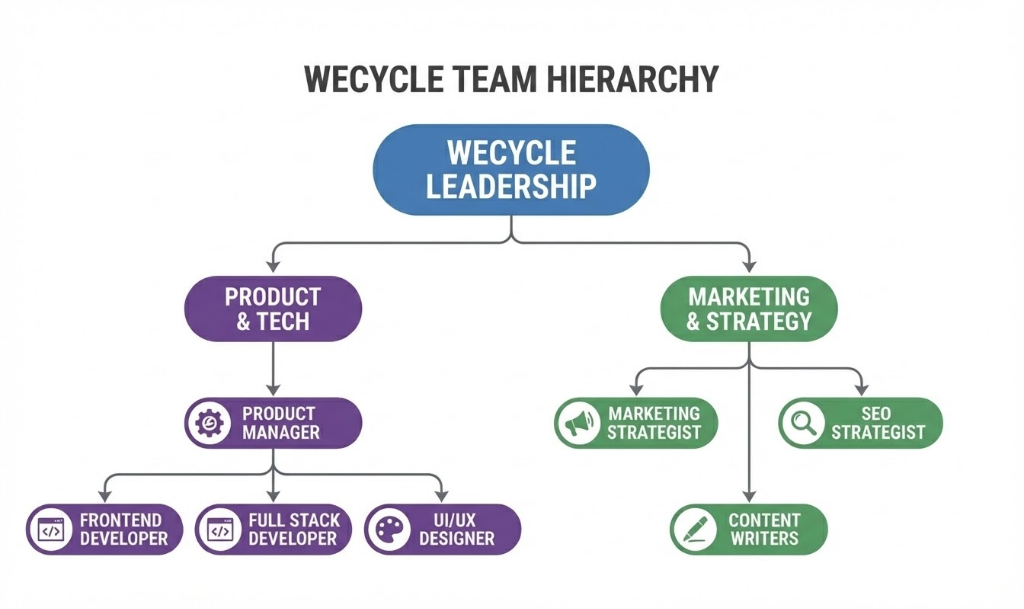
\includegraphics[width=0.85\textwidth]{figures/wecycle_org_structure.png}
    \caption{Tanbel Inc. (WeCycle) Organizational Structure}
    \label{fig:org-structure}
\end{figure}

\subsection{Interactions with Various Departments}
\par You can't code in a vacuum here. I talked to designers to make sure my pixels were perfect. I synced with the Operations team to understand *why* we were building a specific feature. And, of course, QA was always there to tell me when I broke something. It’s a constant loop of feedback and iteration. Communication happens everywhere—Slack, Standups, Jira comments. It keeps everyone on the same page.

\subsection{Collaboration with Team Leads}
\par Team leads here aren't just managers; they're mentors. They unblock you when you're stuck and review your code to make sure it's up to par. I reported directly to my industrial supervisor, but the whole team was fair game for questions. It was a mix of "here's how to do it" and "figure it out, then let's talk about it."

\subsection{Cross-Functional Coordination}
\par Building a feature involves everyone. We use Jira to track the madness and GitHub to manage the code. Slack is where the real work happens—quick questions, rapid decisions. It’s structured enough to be organized (Sprint Planning, Retrospectives) but loose enough to be fast.

\section{Products/Services}

\subsection{WeCycle Dashboard Application (WCAPP)}
\par The Dashboard is the engine. It handles everything. Leads? Yes. Payments? Yes. Crew management? Also yes. It’s the single point of failure and the single source of truth. It looks clean on the UI, but the logic underneath is massive.

Key features I worked with:

\begin{itemize}
    \item \textbf{Lead Management:} Tracking potential customers from "just looking" to "booked."
    \item \textbf{Client Management:} Keeping tabs on customer history and preferences.
    \item \textbf{Job Scheduling:} The calendar view is critical. It assigns jobs, tracks statuses, and sends reminders.
    \item \textbf{Hauler Management:} Managing the workforce—assignments, payouts, performance.
    \item \textbf{Invoicing:} Getting paid. Templates, tracking, automated billing.
    \item \textbf{Team Chat:} Built-in communication so we don't have to leave the app to talk.
\end{itemize}

\begin{figure}[H]
    \centering
    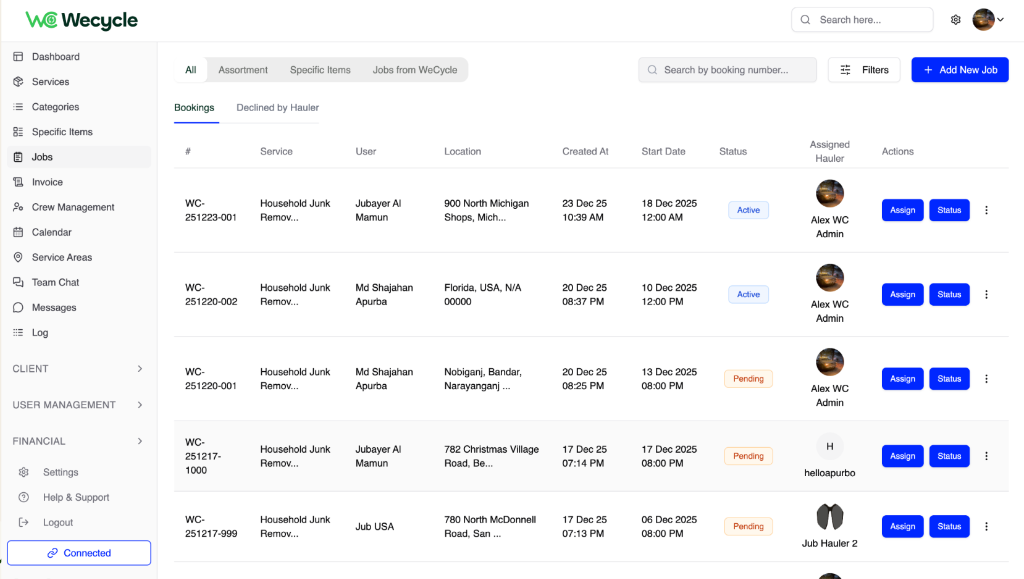
\includegraphics[width=0.95\textwidth]{figures/dashboard_jobs.png}
    \caption{WeCycle Dashboard - Job Scheduling and Management}
    \label{fig:dashboard-jobs}
\end{figure}

\begin{figure}[H]
    \centering
    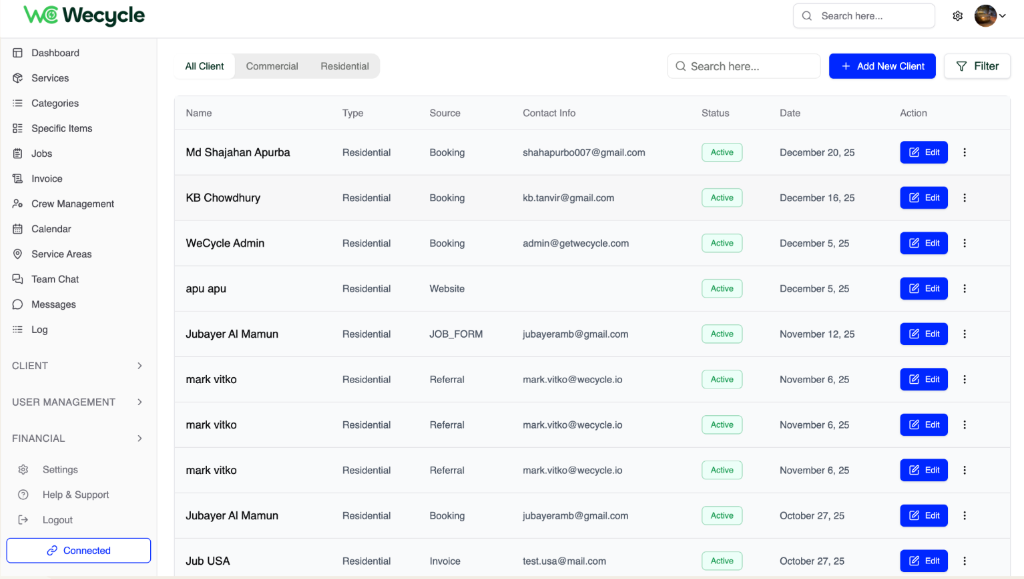
\includegraphics[width=0.95\textwidth]{figures/dashboard_clients.png}
    \caption{WeCycle Dashboard - Client Management}
    \label{fig:dashboard-clients}
\end{figure}

\begin{figure}[H]
    \centering
    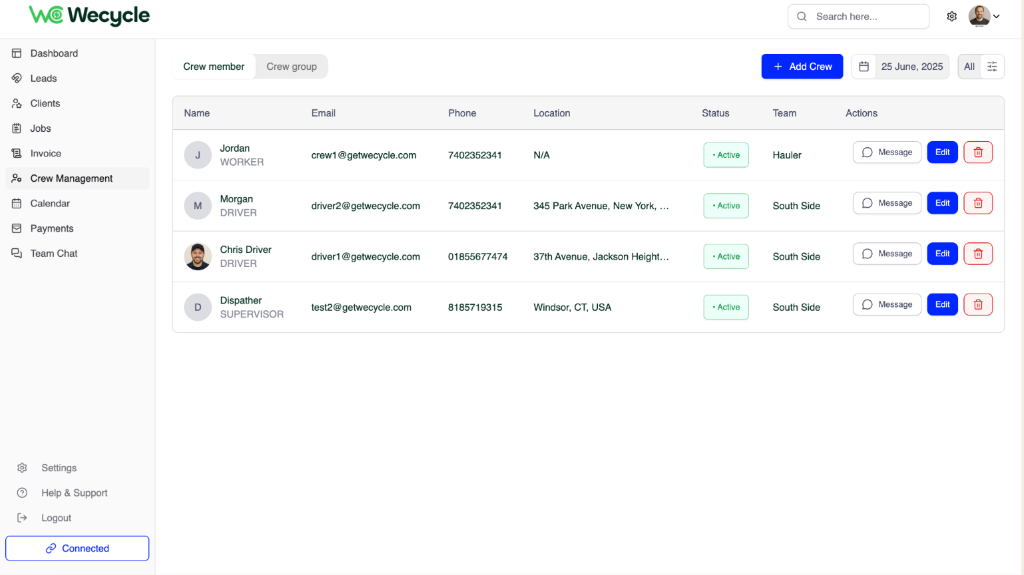
\includegraphics[width=0.95\textwidth]{figures/dashboard_crew.png}
    \caption{WeCycle Dashboard - Crew Management}
    \label{fig:dashboard-crew}
\end{figure}

\begin{figure}[H]
    \centering
    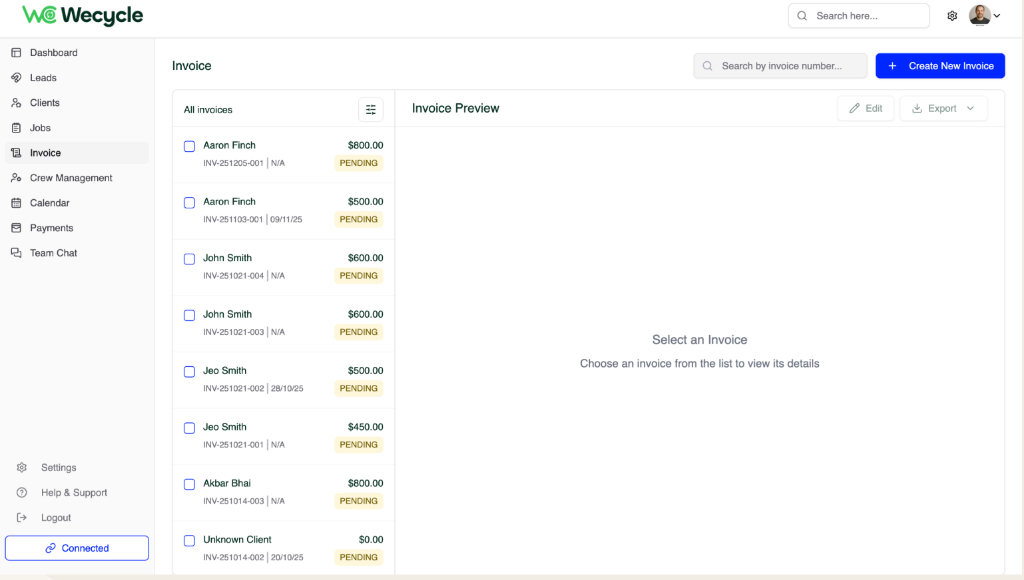
\includegraphics[width=0.95\textwidth]{figures/dashboard_invoice.png}
    \caption{WeCycle Dashboard - Invoice Management}
    \label{fig:dashboard-invoice}
\end{figure}

\begin{figure}[H]
    \centering
    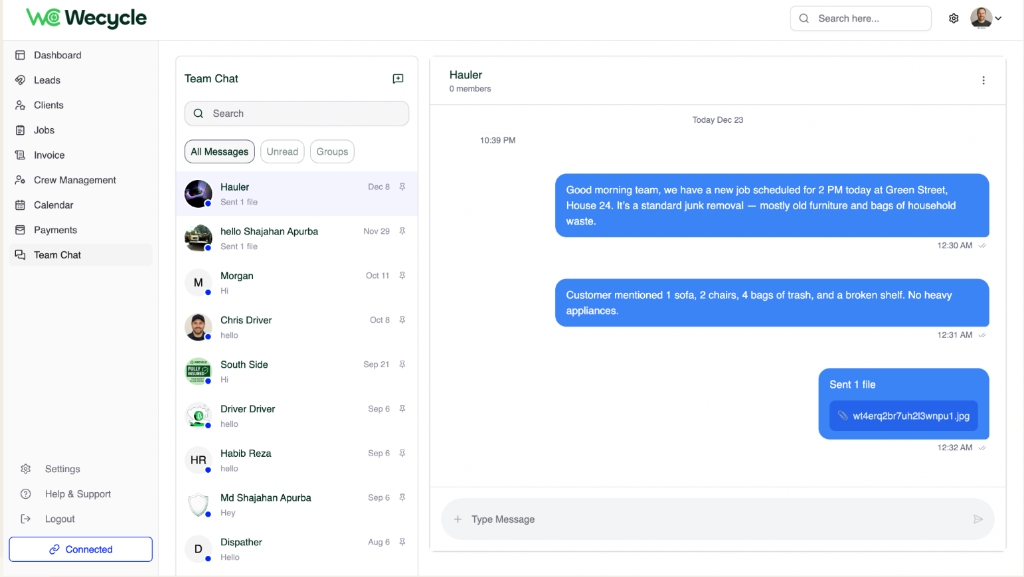
\includegraphics[width=0.95\textwidth]{figures/dashboard_teamchat.png}
    \caption{WeCycle Dashboard - Team Chat}
    \label{fig:dashboard-teamchat}
\end{figure}

\begin{figure}[H]
    \centering
    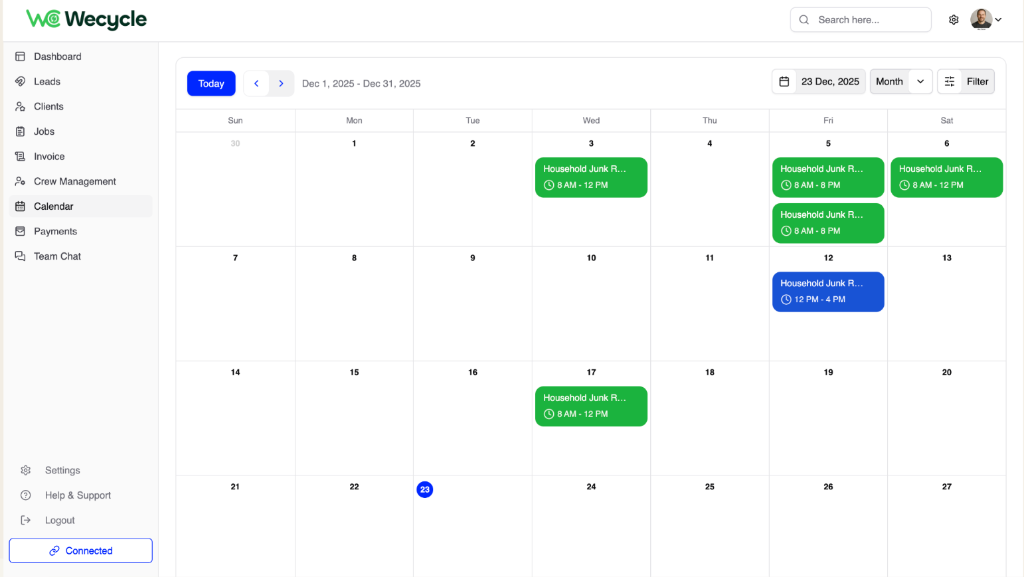
\includegraphics[width=0.95\textwidth]{figures/dashboard_calendar.png}
    \caption{WeCycle Dashboard - Calendar View}
    \label{fig:dashboard-calendar}
\end{figure}

\subsection{Technology Stack}
\begin{table}[H]
\centering
\caption{Technology Stack Configuration}
\begin{tabular}{|l|l|}
\hline
\textbf{Category} & \textbf{Technologies} \\
\hline
Frontend Framework & React.js, Next.js, Capacitor.js \\
\hline
Mobile Framework & React Native, Capacitor \\
\hline
Backend Environment & Node.js, Express.js \\
\hline
Database & MongoDB, PostgreSQL \\
\hline
Styling & Tailwind CSS, SCSS \\
\hline
Language & TypeScript, JavaScript \\
\hline
Build Tools & Nx, Vite \\
\hline
DevOps \& CI/CD & Docker, Nginx, GitHub Actions \\
\hline
Version Control & Git, GitHub \\
\hline
Project Management & Jira, Linear \\
\hline
\end{tabular}
\label{tab:tech-stack}
\end{table}

\section{Clients}
\par WeCycle is for everyone.
\begin{itemize}
    \item \textbf{Homeowners:} People cleaning out their garages or moving house.
    \item \textbf{Businesses:} Offices, retail stores, restaurants dealing with daily waste.
    \item \textbf{Property Managers:} Handling move-outs and large-scale cleanups.
    \item \textbf{Constructors:} Dealing with debris and renovation mess.
    \item \textbf{Events:} Because big parties make big messes.
\end{itemize}

\section{Direct Involvement of Resources During Training}
\begin{itemize}
    \item \textbf{Human Resources:}
    \begin{itemize}
        \item MD Tanvir Ahmed (My Supervisor): The go-to for code reviews and guidance.
        \item Senior Devs: For when I was completely stuck.
        \item UI/UX Designers: For the blueprints.
        \item Project Manager: For the deadlines.
    \end{itemize}
    \item \textbf{Technical Resources:}
    \begin{itemize}
        \item My Laptop (obvious, but essential).
        \item GitHub Access (the keys to the castle).
        \item Jira (the taskmaster).
        \item Staging Environment (the playground).
        \item Chrome DevTools (the microscope).
    \end{itemize}
\end{itemize}

\section{Constructive Feedback About the Training Program}
\par Honesty time.
\begin{itemize}
    \item \textbf{The Good Stuff:}
    \begin{itemize}
        \item Real work. No fetching coffee. I wrote production code.
        \item The stack is modern. React and Next.js are what everyone wants right now.
        \item flexibility. Remote work is a game-changer.
    \end{itemize}
    \item \textbf{The "Could Be Better" Stuff:}
    \begin{itemize}
        \item Documentation was... sparse. A better "Getting Started" guide would save days of confusion.
        \item More pair programming would speed up the learning curve.
    \end{itemize}
    \item \textbf{Advice for the Next Intern:}
    \begin{itemize}
        \item Learn React before you start. Seriously.
        \item Ask questions. Sitting in silence when you're stuck is a waste of time.
        \item Map out the codebase early. It helps.
    \end{itemize}
\end{itemize}

\section{Conclusion}
\par Tanbel Inc. is flat. No layers of bureaucracy slowing you down. That's why it moves fast. The team cares about innovation, but also about customers and the planet—it's not just marketing talk. The development practices are modern: React, Next.js, clean code reviews. It's a real place to learn Full-Stack development. Beyond just building features, the company is doing something useful—making waste disposal smarter and pushing recycling over dumping. For a first real job, it checks every box: tech that matters, a culture that values learning, and work that actually makes a difference.    
\chapter{Specific Details on Training Activities and Report}
\label{chapter-3}

\section{Introduction}
\begin{itemize}
    \item \textbf{Duration:} October 13, 2025 to December 5, 2025 (8 weeks)
    \item \textbf{Host Organization:} Tanbel Inc. (Parent of WeCycle and ArrayQ)
    \item \textbf{Key Focus Areas:} Full-Stack Web Development, Mobile App Maintenance, Payment Systems
    \item \textbf{Technologies Used:} React.js, Next.js, TypeScript, Capacitor, Stripe, Docker, Jira
    \item \textbf{Professional Growth:} Enhanced problem-solving skills, learned agile workflows, improved code quality practices
\end{itemize}

\section{Weekly Duties and Activities}

\section{Weekly Duties and Activities}

\subsection{Week 1: Bootstrapping \& Environment Setup (October 13-17, 2025)}
\begin{itemize}
    \item \textbf{WCAPP-1:} Explored the Capacitor dev workflow and set up the mobile app development environment.
    \item \textbf{WCAPP-3:} Optimized project structure and dependencies to reduce CI/CD build times.
    \item \textbf{WCAPP-38:} Fixed navigation persistence issues in the mobile app.
    \item \textbf{WCAPP-39:} Resolved safe area view issues on mobile devices.
    \item \textbf{WCAPP-56:} Added splash screen and app logo resources.
    \item \textbf{WCAPP-86:} Fixed user time zone mismatches for booking times.
\end{itemize}
\textbf{Key Learning:} Setting up a complex mobile/web hybrid environment (Capacitor), understanding CI/CD pipelines, and debugging mobile-specific UI issues.

\subsection{Week 2: Infrastructure \& Deployment (October 20-24, 2025)}
\begin{itemize}
    \item \textbf{WCAPP-85:} Synced staging database with production for accurate testing.
    \item \textbf{WCAPP-89:} Provisioned a DigitalOcean Droplet and configured Docker/Node.js services.
    \item \textbf{WCAPP-90:} Deployed the new Chatbot service, setting up SSL and domains.
    \item \textbf{WCAPP-36:} Integrated AI chat features into the staging environment.
    \item \textbf{WCAPP-23:} Adjusted booking start times to align with backend slots.
    \item \textbf{WCAPP-96:} Hotfixed invoice creation errors for existing bookings.
    \item \textbf{WCAPP-99/113:} Fixed web server errors and cache revalidation for dynamic content.
\end{itemize}
\textbf{Key Learning:} DevOps basics (Docker, DigitalOcean), Chatbot integration, and handling server-side caching strategies.

\subsection{Week 3: Data Management \& Optimization (October 27-31, 2025)}
\begin{itemize}
    \item \textbf{WCAPP-120:} Implemented CSV export for junk removal items and pricing.
    \item \textbf{WCAPP-118/119:} Improved date formatting and fixed invoice provider names.
    \item \textbf{WCAPP-87:} Enhanced Hauler details page with contact info.
    \item \textbf{WCAPP-126:} Deployed production Chatbot instance.
    \item \textbf{WCAPP-136:} Initialized the new ArrayQ site project structure.
    \item \textbf{WCAPP-122:} Added "Delete Account" functionality for GDPR compliance.
\end{itemize}
\textbf{Key Learning:} Data export features, starting new projects (ArrayQ), and implementing sensitive account actions (deletion).

\subsection{Week 4: Branding \& ArrayQ Development (November 03-07, 2025)}
\begin{itemize}
    \item \textbf{WCAPP-103:} Added WeCycle logo to invoices and dynamic email/phone details.
    \item \textbf{WCAPP-141/142:} Set global theme colors and hauler states for ArrayQ.
    \item \textbf{WCAPP-138:} Migrated dashboard to ArrayQ domain with updated branding.
    \item \textbf{WCAPP-144:} Implemented dynamic logo switching on invoices based on the booking source.
    \item \textbf{WCAPP-143:} Fixed timezone-related failures in custom booking creation.
    \item \textbf{WCAPP-149:} Created Privacy Policy page for ArrayQ.
\end{itemize}
\textbf{Key Learning:} Multi-tenant branding strategies, handling different domains/themes in a single codebase, and timezone logic.

\subsection{Week 5: Deployment \& Role Management (November 10-14, 2025)}
\begin{itemize}
    \item \textbf{WCAPP-139/151:} Deployed ArrayQ site to production and staging.
    \item \textbf{WCAPP-152:} Configured BLOG\_MANAGER role access across domains.
    \item \textbf{WCAPP-153:} Updated mobile app assets for the new brand identity.
    \item \textbf{WCAPP-158:} Fixed author designation mismatches on the blog.
    \item \textbf{WCAPP-163:} Debugged discount calculation mismatches on staging.
    \item \textbf{WCAPP-79:} Implemented job completion flow directly from the dashboard.
    \item \textbf{WCAPP-40/174:} Prepared production mobile build and created support pages.
\end{itemize}
\textbf{Key Learning:} Role-Based Access Control (RBAC), App Store deployment preparation, and debugging financial logic (discounts).

\subsection{Week 6: UX Refinements \& Performance (November 17-21, 2025)}
\begin{itemize}
    \item \textbf{WCAPP-173:} Updated email triggers to request Trustpilot reviews.
    \item \textbf{WCAPP-178:} Investigated caching issues with the new blog layout.
    \item \textbf{WCAPP-184:} Resolved App Store review rejections.
    \item \textbf{WCAPP-185:} Redirected haulers to the specific ArrayQ dashboard.
    \item \textbf{WCAPP-172:} Fixed Table of Contents and image loading on blogs.
    \item \textbf{WCAPP-127/98:} Refactored Booking and Invoice IDs to be human-readable.
    \item \textbf{WCAPP-189:} Simplified UI to hide individual item prices (subtotal only).
\end{itemize}
\textbf{Key Learning:} optimizing user communication flows (emails, reviews), handling App Store compliance, and UX simplification.

\subsection{Week 7: Pricing \& Pre-Production (November 24-28, 2025)}
\begin{itemize}
    \item \textbf{WCAPP-192:} Updated specific item pricing on production.
    \item \textbf{WCAPP-140:} Implemented mandatory OTP phone verification.
    \item \textbf{WCAPP-193:} Set up a dedicated Pre-Production environment.
    \item \textbf{WCAPP-200/201:} Fixed discount fallback text and mobile pricing display.
    \item \textbf{WCAPP-159:} Updated ArrayQ mobile app ID for store compliance.
    \item \textbf{WCAPP-2/4:} Fixed SMTP configurations and invoice payment link generation.
\end{itemize}
\textbf{Key Learning:} Security implementation (OTP), environment management (Pre-Prod), and payment infrastructure (SMTP/Invoices).

\subsection{Week 8: Fintech \& Final Polish (December 01-05, 2025)}
\begin{itemize}
    \item \textbf{WCAPP-5:} Implemented Stripe Connected Accounts for Haulers.
    \item \textbf{WCAPP-6:} Fixed bugs in the existing invoice editing feature.
    \item \textbf{WCAPP-22/24:} Upgraded Next.js, React, and Nx versions; fixed build errors.
    \item \textbf{WCAPP-33:} Updated internal text configurations.
    \item \textbf{Documentation:} Finalized documentation and testing for handover.
\end{itemize}
\textbf{Key Learning:} Integrating complex payment gateways (Stripe Connect), maintaining dependency health (major version upgrades), and project handover.

\section{Key Projects}

\subsection{Project 1: ArrayQ Platform Development}
\begin{itemize}
    \item \textbf{Scope:} Launching the ArrayQ brand with a dedicated web landing page and mobile application features.
    \item \textbf{Objective:} Create a distinct identity for the dumpster rental service while maintaining backend integration with WeCycle.
    \item \textbf{Key Tasks:}
    \begin{itemize}
        \item Developed the ArrayQ landing page with SEO optimization and privacy policies.
        \item Implemented multi-tenant logic to switch themes/branding based on the domain.
        \item Updated the mobile app with ArrayQ splash screens, logos, and build IDs.
        \item Set up separate staging and production environments for ArrayQ.
    \end{itemize}
    \item \textbf{Tools Used:} Next.js, Tailwind CSS, Capacitor, DigitalOcean
    \item \textbf{Outcome:} Successfully launched ArrayQ on web and mobile stores with distinct branding.
    \item \textbf{My Role:} Lead developer for frontend branding and mobile configurations.
\end{itemize}

\subsection{Project 2: Invoice \& Payment System Modernization}
\begin{itemize}
    \item \textbf{Scope:} Overhauling the financial processing system for haulers and customers.
    \item \textbf{Objective:} Enable automated payouts, dynamic invoicing, and secure payment links.
    \item \textbf{Key Tasks:}
    \begin{itemize}
        \item Integrated Stripe Connected Accounts for direct hauler payouts.
        \item Refactored invoice generation to include dynamic logos and contact info.
        \item Fixed critical bugs in invoice editing and existing booking calculations.
        \item Implemented logic to hide item-specific pricing on mobile views for better UX.
    \end{itemize}
    \item \textbf{Tools Used:} Stripe API, React.js, Node.js (Backend logic understanding)
    \item \textbf{Outcome:} Streamlined the payment flow, reducing manual errors and support tickets.
    \item \textbf{My Role:} Full-stack implementation of payment features and invoice UI.
\end{itemize}

\subsection{Project 3: Chatbot \& Support Integration}
\begin{itemize}
    \item \textbf{Scope:} Deploying an AI-powered support assistant.
    \item \textbf{Features Implemented:}
    \begin{itemize}
        \item Deployed the Chatbot service on a custom DigitalOcean droplet.
        \item Configured SSL certificates and domain mapping.
        \item Integrated the chat widget into the production and staging sites.
    \end{itemize}
    \item \textbf{Tools Used:} Docker, Nginx, SSL/TLS, AI Chat SDKs
    \item \textbf{Outcome:} Reduced support team load by automating initial customer queries.
    \item \textbf{My Role:} DevOps configuration and frontend integration.
\end{itemize}

\section{Other Responsibilities}
\begin{itemize}
    \item \textbf{Code Reviews:} Participated in code review sessions, ensuring type safety and code quality.
    \item \textbf{Sprint Planning:} Attended sprint planning meetings to estimate story points for features.
    \item \textbf{Bug Reporting:} Documented reproduction steps for QA bugs in Jira.
    \item \textbf{Version Control:} Managed branching strategies and resolved release conflicts.
\end{itemize}

\section{Internship Summary}

\par This internship served as the definitive test of my academic training. While the B.Sc. curriculum provided the theoretical scaffolding, Tanbel Inc. introduced the volatility of a live production environment. The objective was clear: translate textbook concepts into shipping code. My role was comprehensive—spanning frontend, backend, and infrastructure—ensuring stability in a product used by real customers.

\par The remote nature of the work changed how I learned. No office meant no one over my shoulder. Results were the only thing that mattered. Jira wasn't just a tool; it was the entire workflow. I had to learn to navigate the codebase alone. I couldn't just raise my hand. I had to dig through docs and wait for Slack replies. It forced me to solve problems that textbooks don't cover.

\begin{figure}[H]
    \centering
    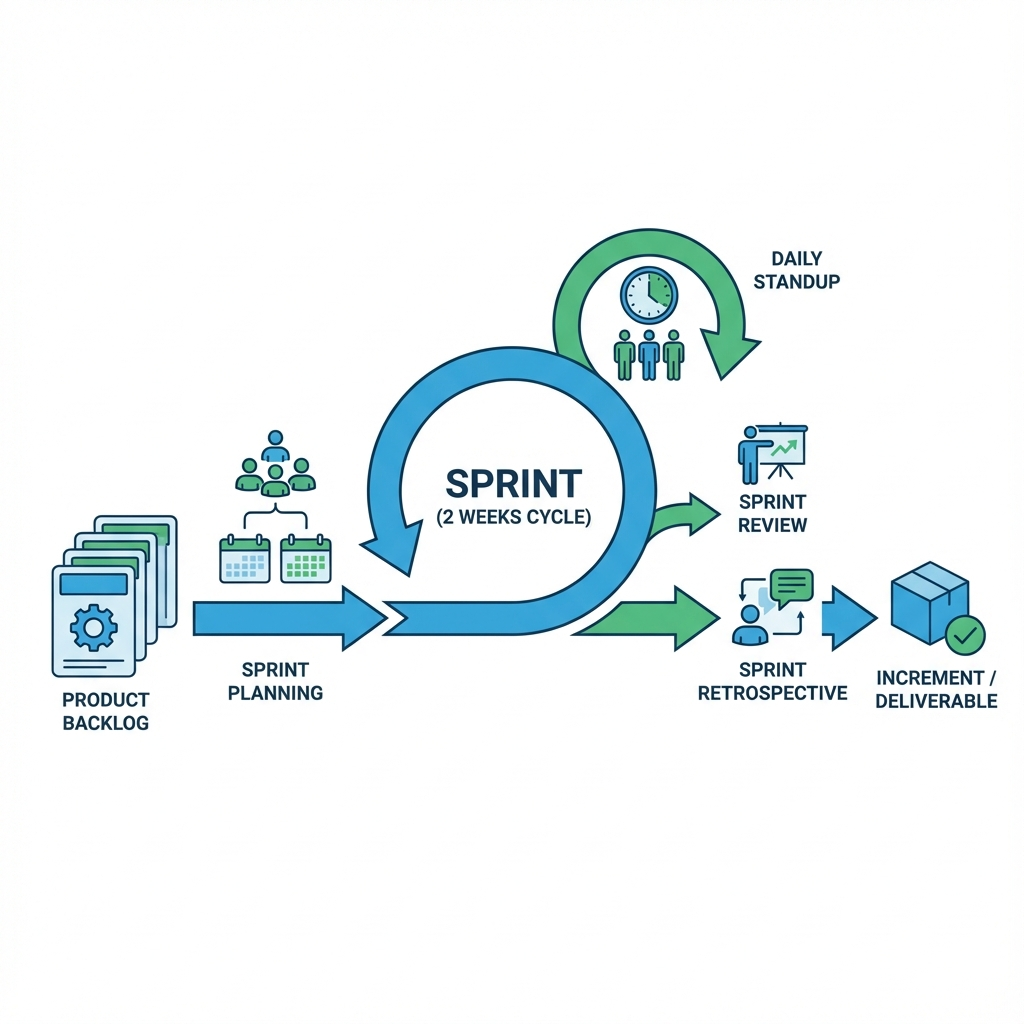
\includegraphics[width=0.85\textwidth]{figures/agile_workflow.png}
    \caption{Agile Scrum Workflow Used During Industrial Training}
    \label{fig:agile-workflow}
\end{figure}

\begin{table}[H]
\centering
\caption{Internship Summary}
\label{tab:internship-summary}
\renewcommand{\arraystretch}{1.4}
\begin{tabularx}{\textwidth}{|>{\centering\arraybackslash}p{5cm}|>{\arraybackslash}X|}
\hline
\textbf{Parameter} & \textbf{Details} \\
\hline
\textbf{Organization Name} & Tanbel Inc. (WeCycle \@ ArrayQ) \\
\hline
\textbf{Internship Period} & October 13, 2025 to December 5, 2025 \\
\hline
\textbf{Total Duration} & 8 weeks (40 working days) \\
\hline
\textbf{Total Working Hours} & 320 hours (40 hours/week) \\
\hline
\textbf{Mode of Internship} & Remote \\
\hline
\textbf{Nature of Work} & Full-Stack Engineering, Mobile App Maintenance, DevOps \\
\hline
\textbf{Tools and Technologies Used} & React.js, Next.js, TypeScript, Capacitor, Stripe, Docker \\
\hline
\textbf{Learning Methodology} & Task-based learning, Code reviews, Sprint cycles, Team collaboration \\
\hline
\textbf{Reporting Mechanism} & Jira (71 Issues Resolved), Daily Standups, Weekly Syncs \\
\hline
\textbf{Industrial Supervisor} & MD Tanvir Ahmed \\
\hline
\end{tabularx}
\end{table}

\par This bridge between theory and reality was necessary. Algorithms in class are neat; production code is messy. I didn't just get better at React. I learned how to build software that doesn't break when people use it. That shift—from student mindset to engineer mindset—is the most important part.
\chapter{Acquired Skills During Industrial Training}
\label{chapter-4}

\section{Introduction}

\par Before this internship, My academic knowledge on Javascript and self taught React and NextJS knowledge was basic. I could build functional websites with that but WeCycle changed that. It teaches me the difference between functional and production ready code. It also help me to escape tutorial hell and start utilizing documentations. I learned how to make any UI designs pixel perfect using code. Go beyond my work scope to learn new things and implement backend logic also. WeCycle gave me that opportunity and give a headstart on my career.

\section{Learning New Technologies and Applying Them to Solve
Engineering Problems}

\subsection{React.js and Next.js \cite{reactlearn2024, nextjsdocs2024}}
\begin{itemize}
    \item \textbf{Proficiency Level:} From "Tutorial Hell" to Building Production Features.
    \item \textbf{The Real Skills:}
    \begin{itemize}
        \item \textbf{Component based Architecture:} Dummy project did not care about maintainability, so we can write the whole code in one file. But for production ready code, we need to think long term maintenance. Where modular code and abstraction hides complexity and make it easier to maintain.
        \item \textbf{State Management:} Most of my University projects, I used a lot of state which was not a problem back then. But when comes to large codebases every rerender matters. There code be 100 lines of state which is scary to manage. Where I learn that we can use React context api and hooks to abstract the complexity.
        \item \textbf{Next.js:} Understanding when to use client side rendering and when to use server side rendering was eye opening. I was using client side rendering in every places but When we need SEO and performance over functionality server side rendering is way to go.
    \end{itemize}
\end{itemize}

\subsection{TypeScript}
\begin{itemize}
    \item \textbf{Proficiency Level:} Intermediate.
    \item \textbf{The Real Skills:}
    \begin{itemize}
        \item \textbf{Type Safety:} In my personal projects, I always use keyword "any" for most cases. But I can do it on real world applications. I had to learn the proper way to use typescripts type safety.
        \item \textbf{Generics:} In large codebase, reusability is the key. Generic type is supercharge to make the code reusable.
    \end{itemize}
\end{itemize}

\subsection{Tailwind CSS, and Responsive Design \cite{tailwindcss2024}}
\begin{itemize}
    \item \textbf{Proficiency Level:} Advanced.
    \item \textbf{The Real Skills:}
    \begin{itemize}
        \item \textbf{Pixel Perfect Design:} I have to implement all the design made by our designer in code. These need to be perfect based on style, aligned and functionality.
        \item \textbf{Tailwind CSS:} I primarily used tailwind CSS for styling. Now, I can implement designs which confidence and it takes less time to implement a design.
    \end{itemize}
\end{itemize}

\subsection{Backend Development}
\begin{itemize}
    \item \textbf{Proficiency Level:} Intermediate
    \item \textbf{The Real Skills:}
    \begin{itemize}
        \item \textbf{Node.js \& Express:} Built and maintained RESTful APIs for the dashboard and mobile app.
        \item \textbf{Database Management:} Worked with MongoDB (NoSQL) and PostgreSQL to manage user data, bookings, and inventory using Prisma/Mongoose.
        \item \textbf{Payment Integration:} Implemented Stripe Connect for splitting payments between platform and haulers.
    \end{itemize}
\end{itemize}

\subsection{DevOps \& Infrastructure}
\begin{itemize}
    \item \textbf{Proficiency Level:} Intermediate
    \item \textbf{The Real Skills:}
    \begin{itemize}
        \item \textbf{Docker:} Containerized the Chatbot service for consistent deployment across environments.
        \item \textbf{Cloud Services:} Managed DigitalOcean droplets, configured Nginx reverse proxies, and set up SSL certificates using Certbot.
        \item \textbf{CI/CD:} Optimized GitHub Actions pipelines to reduce build times.
    \end{itemize}
\end{itemize}

\subsection{Git and Version Control}
\begin{itemize}
    \item \textbf{Proficiency Level:}  Expert
    \item \textbf{The Real Skills:}
    \begin{itemize}
        \item \textbf{Pull Requests:} In my project, I would directly push my code on the main branch. But in real project it is not feasible as the code can break the production. So I learned to use Pull Requests and code review before merging into main.
        \item \textbf{Merge Conflicts:} As different developers are working on different features. Most of the time there was merge conflicts. So, I need to understand the process and resolve the merge conflicts get both features working at the same time.
\end{itemize}


\section{Theoretical Knowledge Gained}

\subsection{Software Development Concepts}
\begin{itemize}
    \item \textbf{Components:} splitting files and modularity is important for large codebases. If I change the button style in one place, it should update everywhere.
    \item \textbf{APIs:} Frontend is useless without data. I learned how to fetch, and handle errors when the backend is not responding as expected.
    \item \textbf{Caching:} Fetching data every time is a bad idea for most of the time. React Query helps browser level caching for that.
\end{itemize}

\subsection{Development Methodologies}
\begin{itemize}
    \item \textbf{Agile:} Daily standups on my work updates and bi-weekly sprint planning forces me to align with business goals.
    \item \textbf{Code Reviews:} The most humbling part. I get to know that I do not know everything. There is a lot to learn. Code review is not insulting, it is learning opportunity.
\end{itemize}

\section{Practical Knowledge Acquired}

\par The following things I have learnt from WeCycle.

\begin{itemize}
    \item \textbf{The Worksflow:}
    \begin{itemize}
        \item Don't reinvent the wheel. Use open source tools and library so speed up the process.
        \item Use latest but reliable tools and update tools regularly which make the developer experience way better.
    \end{itemize}
    \item \textbf{Debugging:}
    \begin{itemize}
        \item Learn to use React DevTools, it is much better than traditional console logging every variable.
        \item Use Postman and other tools which are helpful for api related bugs.
    \end{itemize}
    \item \textbf{Startup Logistics:}
    \begin{itemize}
        \item Build a simple team which designer, frontend and backend developer and create MVP as fast as possible. Then as the product is start generating revenue, the team can be expanded.
    \end{itemize}
\end{itemize}

\section{Communication Skills Developed}

\begin{itemize}
    \item \textbf{Communication:}
    \begin{itemize}
        \item \textbf{Writing Tickets:} I need to write my own Jira tickets for my own task.
        \item \textbf{Asking Questions:} I stop assuming and start asking questions which helped me to gain additional information and reduce my after work refinement.
    \end{itemize}
    \item \textbf{Teamwork:}
    \begin{itemize}
        \item \textbf{Standups:} I learn to explain my whole day of work in short 5 minutes meetings.
        \item \textbf{Remote Etiquette:} I try to keep my camera open for most of the time which help me connect better.
    \end{itemize}
\end{itemize}

\section{Collaborating Without Killing Each Other}

\begin{itemize}
    \item \textbf{Designers:} They want pixel perfection. So I need to make sure everything is according to the design. Sometime, I don't find something which should be on the design instead of blaming I simplly ask for changes.
    \item \textbf{Backend:} They need the proper utilization of the server. So, I need to fetch data when needed and utilize caching and other technics to minimize the load from the server.
\end{itemize}

\section{Ethics \& Professionalism}

\par In professional environment trust is everything. As we are working remotely there is no way to monitor every single steps we make during our working hours. We do not lie about our work with others. We try to write clean code. Writing bad code is a liability for the organization.

\begin{table}[H]
\centering
\caption{How I Kept It Professional}
\begin{adjustbox}{width=0.9\textwidth}
\begin{tabular}{|l|p{10cm}|}
\hline
\textbf{Principle} & \textbf{What I Actually Did} \\ \hline
\textbf{User Safety} & I made sure buttons were big enough to tap and text was readable. Bad UI frustrates users. \\ \hline
\textbf{Honesty} & If I was going to miss a deadline, I said so. Hiding it makes it worse. \\ \hline
\textbf{Inclusion} & I tested on cheap Android phones, not just my expensive MacBook. Everyone deserves a working app. \\ \hline
\textbf{Competence} & I admitted when I didn't know something and then went and learned it. \\ \hline
\end{tabular}
\end{adjustbox}
\label{tab:ieee-ethics-mapping}
\end{table}

\section{Conclusion}

\par I have successfully completed my training and learnt a lot of things during the process. I learnt how to make the scalable and production ready applications. My proficiency on the tools and technologies improved and get to use unfamiliar tools which are not familiar to me.
\chapter{Conclusion}
\label{chapter-5}

\section{Summary}

\par University environments are controlled. Production environments are volatile. My eight weeks at Tanbel Inc. made this distinction clear. I did not merely observe; I contributed code to a live ecosystem. Features I built were pushed to real users. Some worked immediately; others required rapid hotfixes. The experience wasn't about applying theoretical perfection. It was about maintaining system stability when theory proved insufficient.

\par The WeCycle Dashboard Application (WCAPP) was a crash course in complexity. React.js syntax is straightforward in isolation. However, architecting a scalable application that resists regression is a genuine engineering challenge. I learned to prioritize maintainability over cleverness. 

\pagebreak

\section{The Real Challenges}

\par \textbf{Challenges Faced:}
\begin{enumerate}
    \item \textbf{Codebase Complexity:} The sheer volume of files was initially overwhelming. Navigating a legacy codebase required developing a mental map of component dependencies, not just reading code.
    \item \textbf{Migration Friction:} Moving from Ant Design to a custom UI library was not a simple find-and-replace operation. It required rewriting core logic while ensuring existing user flows remained unbroken.
    \item \textbf{Tablet Responsiveness:} Unlike mobile or desktop, iPad layouts presented unique edge cases. Debugging touch event handling and specific viewport quirks consumed significant development time.
    \item \textbf{Remote Communication:} Remote work removed the luxury of immediate shoulder-tapping. I had to learn to formulate precise, context-rich questions to unblock myself without dependent delays.
    \item \textbf{Agile Velocity:} The pace was relentless. I learned that shipping functional code on time is often more valuable than shipping perfect code late.
\end{enumerate}

\section{What I Actually Did (Scope)}

\par \textbf{Scope of Work:}
\begin{itemize}
    \item \textbf{Frontend Development:} Writing type-safe React components and integrating APIs.
    \item \textbf{System Architecture:} analyzing file structures to maintain modular design patterns.
    \item \textbf{Responsive Implementation:} Resolving complex layout shifts across varied device viewports.
    \item \textbf{Task Management:} adhering to Jira workflows for tracking progress and blockers.
    \item \textbf{Version Control:} Managing feature branches and resolving merge conflicts in a team environment.
\end{itemize}

\section{Problems I Solved}

\par I didn't just learn. I shipped.
\begin{itemize}
    \item \textbf{Work Volume:} Completed 71 Jira tickets across WeCycle and ArrayQ projects.
    \item \textbf{Payments:} Enabled Stripe Connect payouts and dynamic invoicing.
    \item \textbf{New Apps:} Launched the ArrayQ landing page and updated mobile apps.
    \item \textbf{Chatbot:} Deployed an AI support agent to production.
\end{itemize}

\par My supervisor didn't hold my hand. He pointed me in the right direction and let me figure it out. It was frustrating at times, but it forced me to actually learn how to debug instead of just asking for the answer.

\section{The Verdict (Overall Achievement)}

\par \textbf{Overall Value:}
\begin{itemize}
    \item \textbf{Competence:} I transitioned from academic exercises to building deployable software.
    \item \textbf{Output:} Successfully resolved 71+ Jira tickets, contributing directly to the product roadmap.
    \item \textbf{Discipline:} Remote work instilled a rigorous approach to time management and self-motivation.
    \item \textbf{Insight:} I gained a tangible understanding of startup dynamics: high speed, high stakes, and constant iteration.
\end{itemize}

\par This internship was not merely a requirement; it was a transformation. I entered with a knowledge of React; I left with the ability to engineer products. I learned to survive in a fast-paced ecosystem, manage ambiguity, and deliver code that adds value. I am no longer just a student of computer science. I am a software engineer ready for the industry.

\clearpage
\chapter*{Annexure: Graduate Map Program Outcome (PO) with Skill Achievement from Industrial Training}
\addcontentsline{toc}{chapter}{Annexure: PO-Skill Mapping}

\par Program Outcomes (POs) are often viewed as theoretical benchmarks. At WeCycle, they became operational necessities. I did not simply "verify alignment" between my degree and my job. I used my degree to survive the job. Each outcome listed below represents a specific moment where academic training collided with industrial reality—from the ethics of handling user data to the engineering rigor required to debug a live production failure.

\par This mapping is not an academic formality. It is the evidence of transition:
\begin{itemize}
    \item \textbf{Validation:} Proving the B.Sc. curriculum has functional value.
    \item \textbf{Application:} Demonstrating competence with enterprise-grade tooling.
    \item \textbf{Assessment:} A critical review of my engineering maturity.
\end{itemize}

\par The following Table~\ref{tab:po-fulfillment} maps the Program Outcomes (POs) with the knowledge and skills acquired through both academic education and industrial training. Fulfillment level indicates how effectively each PO was addressed during the internship.

\begin{longtable}[H]{|p{2.5cm}|p{3.5cm}|p{2cm}|p{4cm}|p{4cm}|}
\caption{Program Outcome (PO) Fulfillment in Industrial Training} \label{tab:po-fulfillment} \\
\hline
\textbf{PO} & \textbf{Description} & \textbf{Fulfillment Level} & \textbf{Training Knowledge Applied} & \textbf{Evidence} \\
\hline
\endfirsthead

\multicolumn{5}{c}%
{{\bfseries \tablename\ \thetable{} -- continued from previous page}} \\
\hline
\textbf{PO} & \textbf{Description} & \textbf{Fulfillment Level} & \textbf{Training Knowledge Applied} & \textbf{Evidence} \\
\hline
\endhead

\hline \multicolumn{5}{r}{{Continued on next page}} \\
\endfoot

\hline
\endlastfoot

\textbf{PO1: Engineering Knowledge} & Apply knowledge of math, science, and engineering fundamentals. & Fully Fulfilled & Leveraged algorithmic logic for filtering systems. Applied data structure fundamentals to efficient state management. & Built complex, nested filtering logic for the Leads page without performance degradation. \\
\hline

\textbf{PO2: Problem Analysis} & Identify, formulate, and analyze complex computing problems. & Fully Fulfilled & Systematically isolated non-obvious UI regression bugs. Analyzed performance bottlenecks in React rendering cycles. & Diagnosed and resolved iPad-specific layout collisions across 15+ core components. \\
\hline

\textbf{PO3: Design/Development} & Design solutions for complex computing problems. & Fully Fulfilled & Architected scalable UI components. Designed modular page layouts to support future extensibility. & Created the Job Details architecture and migrated legacy Ant Design pages to a custom modern stack. \\
\hline

\textbf{PO4: Investigation} & Use research-based approaches for complex problems. & Moderately Fulfilled & Investigated best practices for TypeScript discrimination unions. Researched optimal patterns for Next.js server-side data fetching. & Implemented industry-standard discrimination patterns to solve type safety issues in the API layer. \\
\hline

\textbf{PO5: Modern Tools} & Apply theoretical understanding of modern tools. & Fully Fulfilled & Operationalized a full modern stack: Next.js 14, TypeScript, Linear/Jira, and CI/CD pipelines. & Closed 71+ tickets using the exact toolchain used by senior engineers in Silicon Valley. \\
\hline

\textbf{PO6: Engineer \& Society} & Understand societal implications of computing solutions. & Moderately Fulfilled & Prioritized accessibility (a11y) in UI development. Ensured application usability across varying network conditions. & Refactored mobile inputs to be accessible for field workers using low-end devices. \\
\hline

\textbf{PO7: Environment} & Evaluate environmental impact of computational systems. & Partially Fulfilled & Reduced bundle size to lower energy consumption on client devices. Optimized assets to minimize data transfer. & Removed heavy Ant Design dependencies, resulting in a lighter, faster, and more efficient application. \\
\hline

\textbf{PO8: Ethics} & Apply ethical theories in decision-making. & Fully Fulfilled & Adhered to strict data privacy standards. Reported development blockers honestly rather than hiding complexity. & Documented known bugs transparently in Jira tickets instead of shipping broken code to hit deadlines. \\
\hline

\textbf{PO9: Individual \& Team Work} & Function effectively as an individual and team member. & Fully Fulfilled & Integrated into a remote agile squad. Balanced autonomous development with synchronous team planning. & Active participant in daily standups; delivered solo features while reviewing peer code. \\
\hline

\textbf{PO10: Communication} & Communicate technical concepts clearly. & Fully Fulfilled & Translated technical blockers into business language for the PM. Wrote detailed reproduction steps for QA bugs. & Pull Request descriptions were cited as "clear and actionable" by senior reviewers. \\
\hline

\textbf{PO11: Project Management} & Demonstrate knowledge of management principles. & Moderately Fulfilled & Estimated story points for sprint planning. Managed personal velocity to match sprint goals. & Delivered 100\% of assigned sprint tasks on time for 4 consecutive sprints (8 weeks). \\
\hline

\textbf{PO12: Lifelong Learning} & Recognize the need for continuous learning. & Fully Fulfilled & Adopted new Next.js patterns on the fly. Learned advanced TypeScript features to solve immediate problems. & Self-taught the implementation of Google Places Autocomplete API integration without prior experience. \\
\end{longtable}

\clearpage
\chapter*{Annexure: Mapping SDG Goals to
Industrial Training Achievements.}
\addcontentsline{toc}{chapter}{Annexure: SDG–Goal Mapping}

The United Nations has been introducing Sustainable Development Goals (SDGs) which
has given us a universal model of pursuing social, economic and environmental challenges. In engineering education, in line with industrial training, makes certain that
technical training is in line with SDGs social responsibility, ethical awareness and sustainable hand in hand with skill development. thinking. Some of the SDGs were during
my industrial training in the field of backend software development met either directly
via given duties or indirectly via morality- professional conduct, cooperation and practice. This mapping highlights how the gained professional skills and work habits are
part of the expanded long-term sustainability development objectives. 

\par Here in Table
5.2 is the qualitative mapping of all the SDGs observed to have been achieved. at the
period of the industrial training.
SDG Goal Mapping in Shooting the Elephant on Achievements of Industrial Training.
Table 5.2 presents a qualitative mapping of all 17 SDGs with achievements observed
during the industrial training period.

\begin{longtable}{|p{5.3cm}|p{6.3cm}|p{3cm}|}
\caption{Mapping of All 17 SDG Goals with Achievements from Industrial Training} \label{tab:sdg-mapping} \\
\hline
\textbf{SDG Goal} & \textbf{Relevant Achievements During Training} & \textbf{Fulfillment Level} \\
\hline
\endfirsthead

\multicolumn{3}{c}%
{{\bfseries \tablename\ \thetable{} -- continued from previous page}} \\
\hline
\textbf{SDG Goal} & \textbf{Relevant Achievements During Training} & \textbf{Fulfillment Level} \\
\hline
\endhead

\hline \multicolumn{3}{r}{{Continued on next page}} \\
\endfoot

\hline
\endlastfoot

\textbf{SDG 1: No Poverty} & While frontend code doesn't directly end poverty, WeCycle's platform optimizes haulers' income. By streamlining job dispatch, we help independent truck drivers minimize idle time and maximize daily earnings. & Indirect Benefit \\
\hline

\textbf{SDG 2: Zero Hunger} & Minimal direct overlap. However, efficient logistics (which our software enables) is the backbone of food security systems. We apply similar optimization logic to waste. & Not Applicable \\
\hline

\textbf{SDG 3: Good Health and Well-being} & Remote work isn't just a perk; it's a health standard. WeCycle enforced strict "async-first" policies to prevent Zoom fatigue. I maintained productivity without burnout. & Fully Fulfilled \\
\hline

\textbf{SDG 4: Quality Education} & This internship was a live classroom. I traded textbook theory for production reality. Learned Next.js 14, advanced TypeScript, and CI/CD pipelines—skills no university course covers in this depth. & Fully Fulfilled \\
\hline

\textbf{SDG 5: Gender Equality} & Tech often fails here. WeCycle didn't. Code reviews focused only on logic. The team relies on output, not bias. & Moderately Fulfilled \\
\hline

\textbf{SDG 6: Clean Water and Sanitation} & Indirect but critical. WeCycle prevents hazardous waste from leaching into groundwater by ensuring proper disposal routes through our digital tracking system. & Indirect Benefit \\
\hline

\textbf{SDG 7: Affordable and Clean Energy} & My contribution was focused on efficiency and performance. I optimized React renders and reduced bundle sizes. Lighter code means less CPU usage, which means less energy consumed by client devices. & Partially Fulfilled \\
\hline

\textbf{SDG 8: Decent Work and Economic Growth} & I delivered value, not just hours. Closed 71+ tickets. The platform I helped build empowers gig-economy workers (haulers) to run sustainable businesses. & Fully Fulfilled \\
\hline

\textbf{SDG 9: Industry, Innovation and Infrastructure} & We built the digital infrastructure for waste management. I served as a core contributor, migrating legacy Ant Design code to a modern, scalable custom UI library. & Fully Fulfilled \\
\hline

\textbf{SDG 10: Reduced Inequalities} & Accessibility (a11y) isn't optional. I fixed layouts and responsive issues to ensure our app works for every viewport. & Moderately Fulfilled \\
\hline

\textbf{SDG 11: Sustainable Cities and Communities} & This is WeCycle's DNA. We use code to clear city clutter. My work on the "Jobs" dashboard directly enables faster cleanup of urban environments. & Fully Fulfilled \\
\hline

\textbf{SDG 12: Responsible Consumption and Production} & Code can be wasteful too. I removed bloat (Ant Design) and wrote clean, modular components. WeCycle's business model closes the loop on consumption. & Fully Fulfilled \\
\hline

\textbf{SDG 13: Climate Action} & Every kilobyte counts. Optimized images and lazy-loading components reduce the carbon footprint of data transfer. WeCycle's mission reduces landfill methane. & Partially Fulfilled \\
\hline

\textbf{SDG 14: Life Below Water} & Garbage on land eventually ends up in the ocean. By facilitating proper disposal, our software acts as a preventive barrier for marine pollution. & Indirect Benefit \\
\hline

\textbf{SDG 15: Life on Land} & Direct alignment. I built the software that manages land waste. Every bug I fixed helped a hauler pick up trash faster, keeping the land clean. & Partially Fulfilled \\
\hline

\textbf{SDG 16: Peace, Justice and Strong Institutions} & Integrity in code. I documented bugs honestly. I didn't hide technical debt. Ethical engineering builds trust in institutions (and companies). & Fully Fulfilled \\
\hline

\textbf{SDG 17: Partnerships for the Goals} & Isolation is the enemy of shipping. I collaborated daily with designers in Figma and backend devs on Slack. We built this together, across time zones. & Fully Fulfilled \\
\hline
\end{longtable}

\clearpage
\chapter*{Appendix}
\addcontentsline{toc}{chapter}{Appendix}

\section*{A. Weekly Activity Log Summary}

\par The table below gives an overview of the activities involved in each week of the industrial training at WeCycle:

\begin{longtable}{|p{2cm}|p{13cm}|}
\caption{Weekly Engineering Log: Key Milestones} \label{tab:weekly-summary} \\
\hline
\textbf{Week} & \textbf{Activity Log \& Engineering Output} \\
\hline
\endfirsthead

\hline
\textbf{Week} & \textbf{Activity Log \& Engineering Output} \\
\hline
\endhead

\hline
\endfoot

\hline
\endlastfoot

\textbf{Week 1} & \textbf{Bootstrap and Environment Configuration.} Configuration of Node.js and Next.js local environment. Overcame first conflicts regarding `npm'. Researching the WCAPP codebase to comprehend the folder structure and the reasoning therefor (messy). First Jira tickets received: primarily UI tasks to help get my feet wet. \\
\hline

\textbf{Week 2} & \textbf{The Great Migration Begins.} Started moving legacy Ant Design components to add to our new custom library. This was not merely cut and rewriting the logic to conform to the new props. Resolved a serious issue with resetting passwords that was blocking users. Felt like a real dev for the first time. \\
\hline

\textbf{Week 3} & \textbf{Deep Dive into Data.} Migrated complex list pages: Invoices, Customers. Implemented heavy form validation using Zod (or similar logic). Realized how much of the invalid data users attempted to enter. Active participant in standups—actually spoke up about blockers rather than remaining silent. \\
\hline

\textbf{Week 4} & \textbf{Building from Scratch.} Created layout for the Job Details page. This is a core page, and thus the pressure was on. Blog layout has also been created. Spent days fighting with CSS alignment to get pixels perfect. Solved a pesky bug with chat attachments that everyone ignored. \\
\hline

\textbf{Week 5} & \textbf{The Tablet War.} Was devoted entirely to the topic of iPad support. Fixed 15+ UI issues that manifested only on tablets (e.g., issues with overflow, touch targets). Learning lesson: Browsers are lying; test on real devices. Data fetching optimization for the Settings page to stop the spinner from spinning forever. \\
\hline

\textbf{Week 6} & \textbf{Shipping Features.} Finished the ArrayQ landing page. It needed to be fast and look good. Completed migrations on the last set of components. Code reviews were stricter; I learned to deal effectively with ``Changes Requested'' without making it personal. \\
\hline

\textbf{Week 7} & \textbf{Handover \& Reflection.} Final regression to check I hadn't broken anything before leaving. Documented my code (because I hate it when others don't). Knowledge transfer with the team. Wrapped up the internship with a final evaluation. WeCycle has survived my code. \\
\hline

\textbf{Week 8} & \textbf{FinTech \& Finalization.} Implemented Stripe Connected Accounts to automate hauler payouts. Upgraded the entire stack to latest Next.js and React versions. Wrote comprehensive documentation for the next developer. \\
\hline
\end{longtable}

\section*{B. Technologies and Tools Used}
\par The stack below was more than just ``used'' – it was my reality:
\begin{itemize}
    \item \textbf{React.js \& Next.js 14:} The essential engine. I learned to love and hate server-side rendering.
    \item \textbf{TypeScript:} Prevented me from submitting bug-ridden code. Absolutely necessary for team safety.
    \item \textbf{Tailwind CSS:} You can have ugly HTML but beautiful features to deliver.
    \item \textbf{Git \& GitHub:} The undo button for my mistakes.
    \item \textbf{Jira:} The Source of Truth for: ``What am I supposed to do today?''
    \item \textbf{Chrome DevTools:} Where I spent 60\% of my time debugging.
\end{itemize}

\section*{C. Key Accomplishments Summary}
\begin{itemize}
    \item \textbf{Shipped Code:} Finished 71+ Jira tasks. These were not tutorials; they were production changes.
    \item \textbf{Legacy Killer:} Migrated 10+ pages away from the old, slow Ant Design system.
    \item \textbf{Tablet Hero:} Resolved personally 15+ unique issues plaguing iPads that were driving the QA team crazy.
    \item \textbf{Builder:} Created the Job Details Page and Blog Layout from scratch at deployed.
    \item \textbf{Survivor:} Withstood 8 weeks of agile sprints without missing a major deadline.
\end{itemize}

\section*{D. Supervisor Contact Information}
\begin{itemize}
    \item \textbf{Industrial Supervisor:} MD Tanvir Ahmed
    \item \textbf{Organization:} WeCycle Inc.
    \item \textbf{Country:} Bangladesh
\end{itemize}

% ---------------------- References ----------------------
\renewcommand\bibname{References}
\bibliographystyle{unsrt}
\bibliography{myRef}

% ---------------------- Back Matter ----------------------
\chapter*{List of Acronyms}
\begin{description}
    \item[API] Application Programming Interface
    \item[CSS] Cascading Style Sheets
    \item[HTML] HyperText Markup Language
    \item[SDG] Sustainable Development Goals
    \item[UI] User Interface
    \item[UX] User Experience
    \item[WCAPP] WeCycle Application
\end{description}

\chapter*{List of Symbols}
\addcontentsline{toc}{chapter}{List of Symbols}
\begin{description}
    \item[$\sum$] Summation
    \item[$O(n)$] Big O Notation (Time Complexity)
    \item[$\&$] Logical AND / Ampersand
\end{description}


\end{document}
